\documentclass[11pt]{lecturenotes}

%\let\theenumiorg\theenumi
%
%\newcommand{\code}[1]{\texttt{#1}}
\topsep 0pt

\usepackage{enumitem}

\newcommand{\objExplainPrinciples}{\item explain the principles of survey design including question design, sampling, statistical inference, and sources of error}
\newcommand{\objDevelopQuestions}{\item explain the principles of survey design including question design, sampling, statistical inference, and sources of error}
\newcommand{\objAdvocate}{\item advocate for inclusion of measures on surveys using a scientific justification}
\newcommand{\objDataManagement}{\item conduct basic data management tasks and descriptive analysis in \textsf{R}}


\title{Survey Questions and Answers}
\author{Michael Bader}
\week{6}
\lesson{1}
\coursenumber{SOCY 625}
\coursetitle{Practicum in Sociological Research}


\begin{document}
\maketitle

\begin{objectives}{
\item Describe the cognitive model used to respond to survey questions
\item Identify and describe problems that arise when respondents answer survey questions 
\item Enumerate good question design principles
}{
\objExplainPrinciples
\objDevelopQuestions
}
\end{objectives}

\section{Asking Questions in a Survey Setting}
\subsection[15]{Review Measurement Inference}
Having finished the first workshop offers us a chance to review where we have been and look forward to where we are going. 

\slide
Let's recall, what types of questions can survey research help us answer?\\
$\longrightarrow$ Questions about the prevalence of some social phenomenon in a representative population

In order to do that, we need to \textbf{infer} population-level characteristics based on: 
\begin{enumerate}[label=\Alph*]
\item Measurement inference (response$\rightarrow$construct)
\item Representational inference (sample$\rightarrow$population)
\end{enumerate}

As I mentioned before, we will be spending the next part of the class working on minimizing measurement errors. Therefore, we will be working on the left side of this figure: \slide

\begin{center}
\includegraphics[scale=.5]{../../Week2-InferenceAndError/images/GrovesCh2Fig2.pdf}
\end{center}

In particular, we are going to be working on assessing the \emph{validity} of our measures, which for us will come from survey questionnaires

\subsection[5]{Survey Context}
\slide
It's important to remember that we collect data in a particular context. For the DCAS, we will be using a self-administered paper and pencil interview (PAPI). We won't spend a long time discussing the other modes, but you should be aware of some: 

\begin{description}
\item[PAPI] Paper and pencil interview
\item[CAPI] Computer-assisted personal interview
\item[SAPI] Self-administered personal interview
\item[WAPI] Web-assisted personal interview
\end{description}

In the context of interviews administered by interviewers, the practice of interviewing someone takes on something like a very stilted conversation. When we consider how people respond, there will be something akin to a conversation, and that will affect how respondents respond to questions; but, at the same time, it won't follow the normal conventions of a conversation. 

Similarly, when respondents complete a self-administered survey, the process will ``feel'' like other types of actions for the respondent. We need to conceive of what those might be and how they might affect the manner in which the respondent responds to the survey. What else feels like a self-administered survey? 

\subsection[10]{Encoding}
\slide
We also need to consider how people come to think about the world in order to answer the questions that we ask them. Throughout today, I will break questions down into two broad categories: 
\begin{itemize}
\item behavioral 
\item attitudinal
\end{itemize}

Encoding is the cognitive processes that our minds go through in order to ``make memories.''

\textbf{Events\slash Behaviors}\\
When an event happens and it has some salience to us, we preserve it in long-term memory. When we need it, we retrieve the information related to that event from our memory. 

We can think of information being encoded according to its \textbf{salience}, or how much it means to us, and its \textbf{frequency}, how often the events, or events like it, happen to us.

\textbf{Attitudes}\\
We can think about a similar, though less defined process, for attitudes. We have things happen to us that make us think and feel a certain way. Those get stored in neurons somewhere in our brains. Then, when we experience some stimulus that requires that we describe sentiments based on those experiences and emotions, we can try to describe them. 

When we ask survey questions, we are effectively asking respondents to retrieve information from their memories based on the questions that we ask to answer a question that will help us measure a given \emph{construct}.

\subsection[15]{Cognitive Model}  
To understand how respondents respond to surveys, we should have some cognitive model about what's happening. The one that Groves, et al.\ use is the following: 

\begin{center}\slide
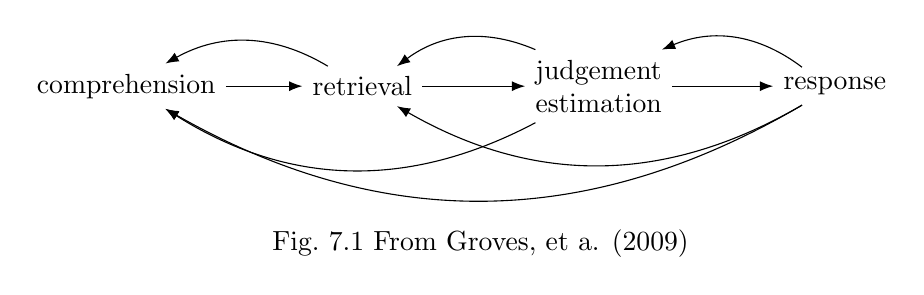
\begin{tikzpicture}
\usetikzlibrary{arrows.meta}

\node [align=center, thick] (comp)  at (0,0) {comprehension};
\node [align=center, thick] (retr) at (3,0) {retrieval};
\node [align=center, thick] (judg) at (6,0) {judgement\\estimation};
\node [align=center, thick] (resp) at (9,0) {response};

\path [-Latex] (comp) edge (retr) (retr) edge (judg) (judg) edge (resp);
\draw [-Latex] (resp) to [bend right] (judg);
\draw [-Latex] (judg) to [bend right] (retr);
\draw [-Latex] (retr) to [bend right] (comp);
\draw [-Latex] (resp) to [bend left] (retr);
\draw [-Latex] (judg) to [bend left] (comp);
\draw [-Latex] (resp) to [bend left] (comp);

\node [align=center] at (4.5,-2) {Fig.\ 7.1 From Groves, et a. (2009)};

\end{tikzpicture}
\end{center}

This model suggests that respondents go through four different stages to answer a question once asked \emph{and} that the process may ``restart'' or ``return'' at any previous stage. 

What we will do for most of the remainder of class is to go through each of these steps, discuss what each is and talk about what errors might come about at that step. 

\section{Errors in Answering Questions}
\subsection[15]{Comprehension}
\slide
\concept{comprehension}{a \emph{respondent's} understanding of the question}

Affected by factors: 
\begin{itemize}
\item \textbf{internal to the question}: understanding the words, knowing what is being ask, being able to retain relevant information from the question
\item \textbf{external to the question}: interpreting the \emph{intent} of the question; inferring the domain of possible answers. 
\end{itemize}

\slide
(create a slide for each item;\\ and for each of the types of errors below, ask the students to think of how their question might have this problem)

\textbf{Problems:}
\begin{description}[topsep=-1em]
\item[Grammar] ambiguity arises from different interpretations of question
\item[Excessive complexity] respondent has difficulty retaining relevant question information in mind to answer question
\item[Faulty presupposition] assumes some state of the world that may not be true
\item[Vague concepts or quantifiers] respondents may differ on meaning of question or response categories
\item[Unfamiliar terms] refers to something that a respondent might not recognize
\item[False inference] respondents try to figure out what a question is ``really'' asking
\end{description}

\subsection[25]{Retrieval}
\slide
\concept{retrieval}{the process of recalling information relevant to answering the question from long-term memory, Groves, et al.\ 221}

Retrieval relates to three basic concepts: 
\begin{itemize}
\item Salience of the event 
\item Frequency of event 
\item Elapsed time since the event
\end{itemize}

\textbf{Problems}\\
We don't actually remember ``events.'' We create a cluster of experiences over time that we treat as events in our minds. What we remember has actually come about through the construction of those events over time by replaying and remembering different parts, supplemented by outside material (e.g., videos, others' recollections, documents, etc.)

\begin{itemize}
\item We fail to gather a memory from our memory bank (faulty memory or because the words that we use to ask the question do not match the words that we used to encode the information to memory)
\item We create a ``generic memory'' for something that occurs frequently that does not have high salience
\item Filling in what we normally do (or \emph{think} that we normally do) to answer a question (reconstruction)
\item Passage of time
\item Telescoping (thinking that events were more recent than they actually are)
\end{itemize}

\concept{measurement (error) model}{a statistical depiction of a process that generates error}

Groves, et al.\ present this \emph{measurement model}:

\[y_i = \mu_i\left(ae^{-bt}\right) + \epsilon_i \]

\begin{description}
\item[$\mu_i$] number of events experienced by the $i$th respondent
\item[$y_i$] report of respondent $i$ to the question
\item[$a$] proportion of events that are reported
\item[$b$] rate of decline in reporting events over time
\end{description}

\textbf{Solutions}\\
You can give the respondent a reference period to help them reconstruct the event in their head 

A strong form of this would be to bound the question based on previous or known information, but it's possible that respondents ``telescope'' their answers and don't fit it to the response period particularly well. 

Use salient or distinct events to anchor memories (life history tables)

\subsection[20]{Estimation}
\concept{estimation}{process of combining or supplementing what the respondent has retrieved}

\emph{Estimation} relates to behavioral questions

\emph{Judgment} relates to attitudinal questions

\slide
\textbf{Estimation}\\
People use three strategies to estimate behaviors\\
\begin{minipage}{.75\textwidth}
\begin{description}
\item[Recall \& count] respondent will try to recall all of the times that they engaged in the behavior during the \emph{reference period} and count those events
\item[Rate-based] respondent will create a rate about how often per some unit of time and then multiply that by the \emph{reference period}
\item[Impression-based] respondents will create an impression of how often they do something
\end{description}
\end{minipage}%
\begin{minipage}{.24\textwidth}
\begin{center}
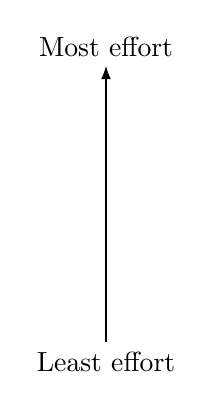
\begin{tikzpicture}
\usetikzlibrary{arrows.meta}
\node [align=center] (least)  at (0,0) {Least effort};
\node [align=center] (most) at (0,4) {Most effort};
\path [-Latex] (least) edge (most);
\end{tikzpicture}
\end{center}
\end{minipage}

Can use a couple different types of responses:
\begin{itemize}
\item Open-ended numeric
\item Closed with ordinal scale (prone to primacy and re\-cen\-cy effects)
\item Closed with categorical scale (prone to primacy and re\-cen\-cy effects)
\end{itemize}

\concept{primacy effect}{people tend to benchmark ideas to the first response that they encounter and base judgments on that first option}

\concept{recency effect}{people tend to respond more to the \emph{last} response given}

In addition, response categories provide strong suggestive evidence to respondents about appropriate ranges, especially for impression-based response estimation strategies. You should be very careful when designing response categories, if you use response categories. 

Judgment-based questions have similar issues, but will be based on how respondents judge the relevance of a topic. They can use a very logical deduction, base it on a quick calculation of other topics or how often they thought about it, or they can develop an answer based on impressions. 

\concept{acquiescence effect}{people tend to like to agree more than they like to disagree}

\section{Writing Good Questions}
Now that we have talked about all of the problems that can arise in asking questions, we should consider how we minimize those errors and ask \emph{good} questions.

\subsection[15]{Nonsensitive Questions about Behavior}
On page 243, Groves, et al. write out a list of guidelines (a checklist of sorts) for evaluating behavior-related questions on non-sensitive topics

\begin{enumerate}[noitemsep]
\item Create comprehensive and mutually exclusive response categories
\item Make question as specific as possible
\item Use familiar words
\item Lengthen questions to add memory cues to improve recall (suggest to respondent what you want them to consider)
\item When forgetting is likely, use aided recall (e.g. use subcategories to questions)\hrule\vspace{.3em}
\item Use a diary
\item Use a life history calendar
\item Ask respondent to use household records to confirm answers
\item Allow a proxy to report for the respondent
\end{enumerate}

\subsection[10]{Sensitive Questions about Behavior}
On page 246, Groves, et al.\ write out a list of guidelines for questions about sensitive behaviors

\begin{enumerate}[noitemsep]
\item Use open rather than closed questions for eliciting the frequency of sensitive behaviors
\item Use long rather than short questions
\item Use familiar words
\item Deliberately load the question to reduce misreporting (write something that shows that certain behaviors are ``okay'' to reduce motivated misreporting)
\item Ask about long periods before asking about more recent behaviors
\item Embed sensitive question among other sensitive items to make it stand out less
\item Add items to assess the sensitivity of behavioral items
\hrule\vspace{.3em}
\item Allow the respondent to administer the survey to him-\slash herself 
\item Collect data in a diary
\item Collect validation data 
\end{enumerate}

\subsection[20]{Attitude Questions}
On page 248, Groves, et al.\ write out a list of guidelines for attitude questions
\begin{enumerate}[noitemsep]
\item Specify the attitude object clearly
\item Measure the strength of the attitude, if necessary using separate items (to avoid double-barreled questions)
\item Use bipolar items except when they might miss key information
\item Carefully consider the alternatives mentioned in the question (they have a big impact on the answers)
\item In measuring change over time or over different groups, ask the same questions
\item When asking both general and specific questions about a topic, ask general items first
\item When asking about multiple items, start with the least popular one
\item Use closed questions for measuring attitudes
\item Use five- or seven-point scales and label every point
\item Start with the end of the scale that is least popular
\item Use analog devices (such as thermometers) to collect more detailed scale information
\item Use ranking only if the respondents can see all alternatives; otherwise use pair-wise comparisons
\item Get ratings for every item of interest; do not use check-all-that-apply items
\end{enumerate}

\slide
\concept{double-barreled question}{questions that ask about two attitudes simultaneously}

Double-barreled questions are, in my experience, the most frequent problem on surveys. We should be careful that we don't inadvertently add our own presuppositions to the question. 

Question from the book on page 249:\\
\textit{Do you favor legalized abortion because it gives women the right to choose?}

If someone answers ``yes,'' do we know if they support legalized abortion? do we know if they support a woman's right to choose? do we know if they support both? 

\slide 
\concept{bipolar approach}{questions that ask respondents to choose between plausible alternatives}

Rather than asking if someone agrees with a statement, we should ask which of two alternatives does a respondent favor more. This reduces acquiescence bias and also elicits more information about where someone stands on an issue.

\end{document}